\section{Overview}
The communications module class, \textit{CommMod}, is the part of the simulator solution that is responsible for performing tasks at level three of the OSI model (the networking layer). Depending on the noise function used by the simulator, it is also possible to have communications modules perform tasks in layer two (such as collision detection and avoidance). Whilst the base class is a part of the simulator itself, the actual implementation of routing algorithms are part of a separate library in their own right. In this way, the communications library is intended to be distributed with \textbf{octoDrone} without being a required constituent part.

\section{Structure}
\subsection{Structure of an Individual Module}
\subsubsection{Sending and Receiving Messages}
		
When a communications module wishes to transmit a message to other units it invokes the broadcast method exposed by the simulation environment. Messages that originate from the communication modules messageable collect in a queue, which must be checked at regular intervals. When there is a message that the environment determines should be delivered to the communications module, it is deposited in a similar queue. When the module has a message it needs to pass to its messageable, it stores it in a third queue.

In addition to asynchronous messaging, the project design also called for synchronous message passing. This is achieved by having a callback function in the messagable which can be invoked upon receipt of an urgent communication. It is left to the communication implementation to decide which messages are important to interrupt the normal operation of the messageable for.
		
\subsubsection{Intermediate Processing}
The virtual function \textit{comm_function} is called when the communications module is started and is expected to return when the associated program is ready to terminate. It should be used to perform any intermediate and non-delivery driven processing such as routing or time based commands.
		
\subsection{Structure of a Collection of Modules}
	
In order to facilitate easy distribution and use, collections of communication implementations are combined into libraries. Given the small size of a communications modules source code (often tens of kilobytes) it might be tempting to statically link them to simulation executables. The problem with this approach, however, is that it precludes the very thing that prompted the creation of communications modules in the first place - modularity. As such, communications code is packaged into a shared library which simulator executables are then linked against dynamically at compile time. This reduces the size of produced executables and makes updating communications code possible without requiring simulations to be recompiled.

\subsection{Access to Other Simulation Elements}
		
The architecture of the simulator requires that communications modules are able to interact with the simulator environment (to dispatch messages), as well as with the messageable with which they are associated. Since it is impossible to have all of this information available when the communications module is instantiated (creating a messageable requires a reference to a communications module as well), it is necessary to set the messageable associated with a communications object at a later time (but before the simulation is started). Thus, the procedure for bootstrapping a simulations is broadly as follows:

\begin{enumerate}
	\item Load the sensor data
	\item Create a simulation environment referencing the sensor data
	\item Create a communications module referencing the environment
	\item Create a messageable referencing the environment and the communications module
	\item Add a reference to the messageable to the communications module
\end{enumerate}

How these references are used is covered in sections \ref{int-sim} and \ref{int-pro}.

\section{Integration with Other Components}

\subsection{Integration with the Simulator}
\label{int-sim}
The communications module class makes use of the following functions from the simulator:

\begin{itemize}
\item \textit{broadcast}
\end{itemize}

\subsection{Integration with a Program}
\label{int-pro}
Programs for drones and base stations can make use of the following functions from \textit{CommMod}:

\begin{itemize}
\item \textit{push_in_message}
\item \textit{push_out_message}
\item \textit{comm_function} (to start the CommMod)
\item \textit{set_messageable} (used when defining simulations)
\end{itemize}

\section{Provided Implementations}
\begin{figure}
\centering
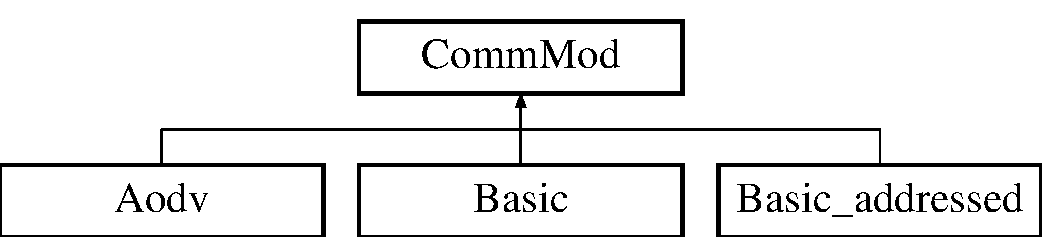
\includegraphics[scale=0.4]{../documentation/latex/class_comm_mod}	
\caption{Inheritance diagram for the \textit{CommMod} class}
\end{figure}

\subsection{Basic Messaging}
\begin{figure}[H]
\centering
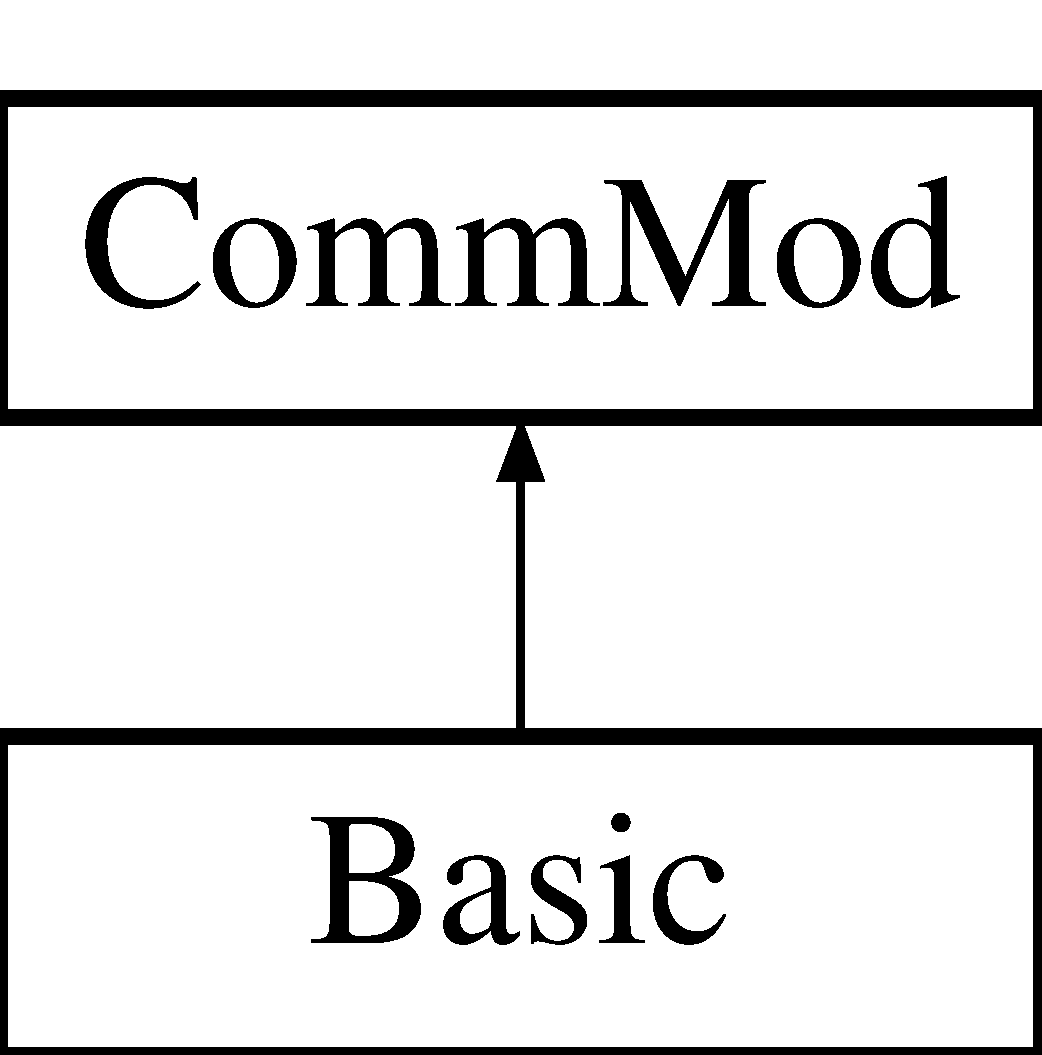
\includegraphics[scale=0.2]{../documentation/latex/class_basic}	
\caption{Inheritance diagram for the \textit{Basic} class}
\end{figure}

The basic messaging implementation provides the simplest possible way of sending and receiving messages. This can be useful when creating programs for messageable units, as it removes the need to consider routing problems, units being out of range, and a whole host of other potential issues. Additionally, it provides a good method for simulating existing programs which were not written with \textbf{octoDrone} in mind and may perform their own addressing.

In this implementation, all messages that are sent are received by all nodes, regardless of range. Messages sent include payload information, but do not store information on the sender or receiver.
	
\subsection{Addressed Basic Messaging}
\begin{figure}
\centering
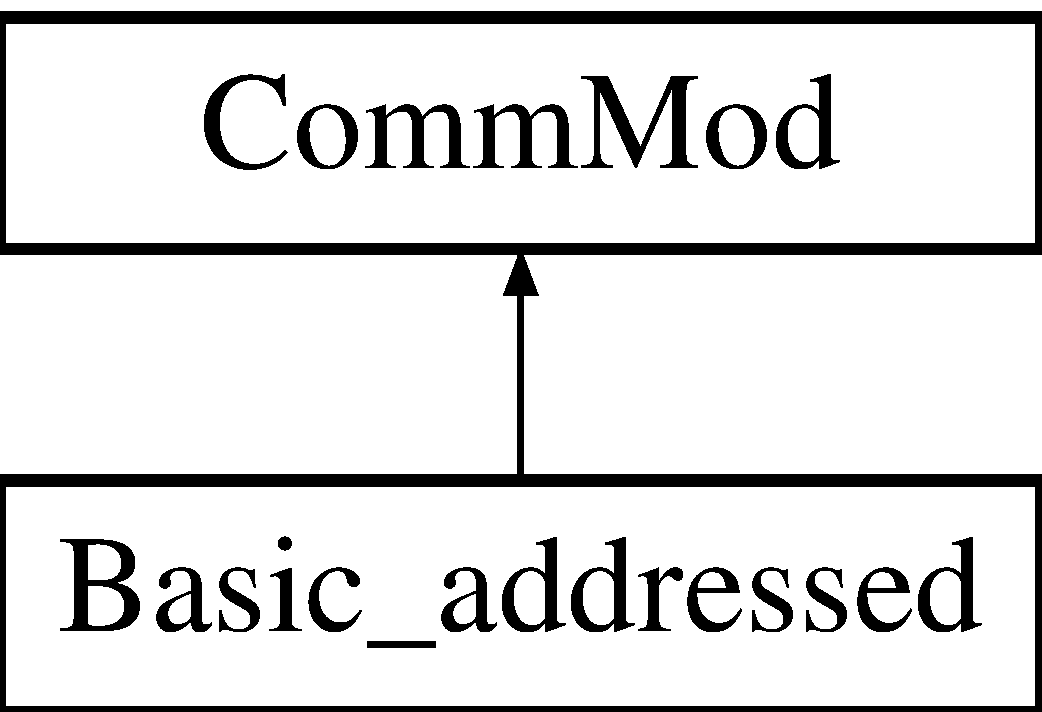
\includegraphics[scale=0.2]{../documentation/latex/class_basic__addressed}	
\caption{Inheritance diagram for the \textit{Basic\_addressed} class}
\end{figure}

The addressed basic messaging implementation extends the above algorithm to additionally take into account the sender and intended recipient of a message when choosing which packets to deliver and which to drop. It is intended to be used for passing messages between programs and communication modules in a way which prevents the need to include code to serialise and deserialise addresses. If appropriate, it can also be used with external programs as described above.

In this implementation, all messages that are sent to an IP address are received by all nodes with that IP address, regardless of range. Messages include payload information as well as the ip addresses of the sender and intended recipient. Messages sent to the broadcast address 255.255.255.0 will be received by all nodes in the simulation.	
	
\subsection{Ad hoc On-Demand Distance Vector Routing}
\begin{figure}
\centering	
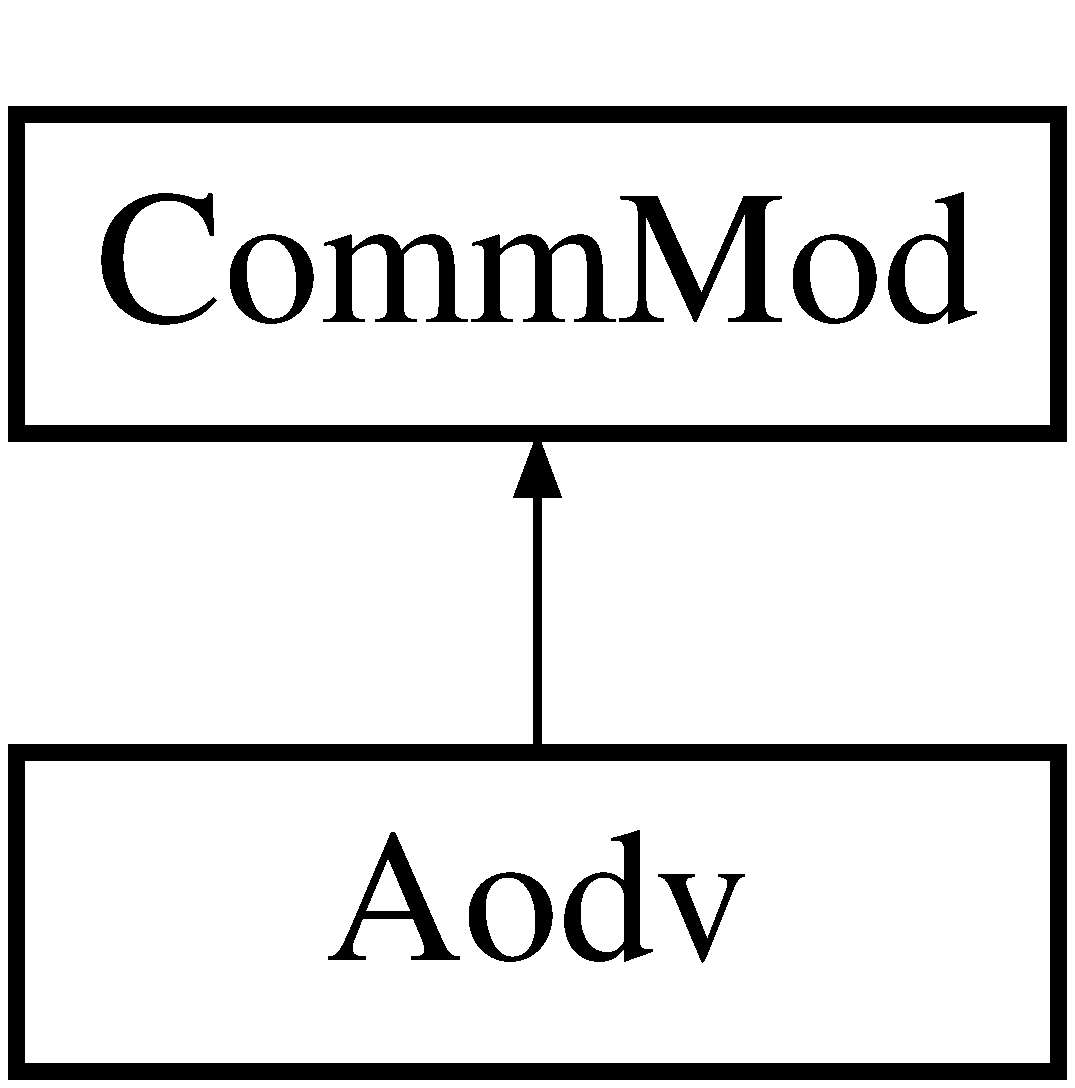
\includegraphics[scale=0.2]{../documentation/latex/class_aodv}	
\caption{Inheritance diagram for the \textit{Aodv} class}
\end{figure}

The Ad hoc On-Demand Distance Vector Routing (AODV) implementation provided in the communications library provides an example of how a more sophisticated routing algorithm can be used within the simulator framework. AODV is designed to be used in mobile ad hoc networks and offers loop free, just in time routing that is fault tolerant and capable of reacting to the movement of nodes.

\subsubsection{Overview}
In order to explain what is happening under the hood of the AODV implementation provided with \textbf{octoDrone} it will be useful to first cover the basics of how the algorithm operates. A node A which wishes to send a data packet to node D 